% !TEX root = ../main.tex
%
\section{Introduction}
\label{sec:introduction}

Research on conversational moderation/facilitation techniques (distinct from “content moderation”, which involves flagging and removing content) is crucial for adapting to evolving online environments, but lags significantly behind current demands \cite{seering_self_moderation, make_reddit_great}. A major challenge lies in the substantial costs required both in researching and moderating discussions, due to human participation \cite{rossi_2024}. Many platforms overcome this by outsourcing moderation to volunteers or users \cite{Matias2019TheCL, schaffner_community_guidelines}, while others turn to content moderation using traditional \ac{ML} models, which are not enough in practice \cite{horta_automated_moderation, schaffner_community_guidelines}. \acfp{LLM} have been hypothesized to be capable of conversational moderation and facilitation tasks \cite{small-polis-llm, korre2025evaluation}. While studies exist for simulating user interactions in social media \cite{park_simulacra, mou_2024, tornberg_2023, y_social, balog_2024}, and for using synthetic moderators \cite{kim_et_al_chatbot, cho-etal-2024-language}, none so far have combined the two approaches. 

\begin{figure}[hbt!]
	\centering
	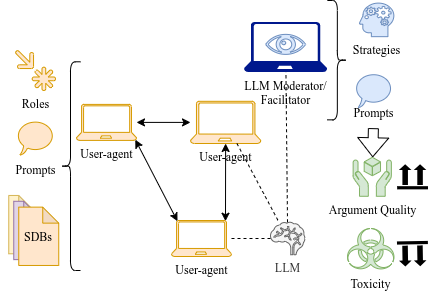
\includegraphics[width=\columnwidth]{research_goal.png}
	\caption{The \ac{LLM} user-agents conduct a discussion, while the \ac{LLM} moderator monitors and attempts to increase its quality. We need to design prompts and configurations for both.}
	\label{fig::goals}
\end{figure}


We propose a simple and generalizable approach using \ac{LLM}-driven synthetic experiments for online moderation research, enabling fast and inexpensive model “debugging” and parameter testing (e.g., selection of prompts, \ac{LLM} moderator instructions) without human involvement (Section~\ref{sec:methodology}) (Fig.~\ref{fig::goals}). We conduct an ablation study (Section~\ref{ssec:results:ablation}), demonstrating that each step of our methodology meaningfully contributes to generating high-quality synthetic data, as well as examining the output of various \acp{LLM}. We do not make the claim that the behavior of \ac{LLM} user-agents is representative of human behavior, as this claim can be scarcely made in Social Science studies involving \ac{LLM} test subjects—we discuss this subject in depth in Section~\ref{ssec:related:human-llm}. Using this methodology, we examine four \ac{LLM} moderation strategies based on current Social Science facilitation research (Section~\ref{sec:experimental})
%: \ac{LLM} alignment guidelines \cite{collective_constitution}, prompts based on human facilitation guidelines \cite{Cornell_eRulemaking2017, dimitra-book} and our own prompt based on \ac{RL} (although we do not perform \ac{RL} in this paper). We 
and compare them with two baselines. We then evaluate these discussions using \ac{LLM} annotator-agents. We use open-source \acp{LLM} and include all relevant configurations in order to make our study as reproducible as possible (see Appendix \ref{ssec:appendix:annotation}, \ref{ssec:appendix:prompts}).


 Our analysis reveals two key findings (Section \ref{sec:results}): (1) the presence of \ac{LLM} moderators exhibited a positive and statistically significant influence on the quality of synthetic discussions, and (2) current moderation strategies are often not enough to meaningfully outperform simple baselines. %However, besides helping in understanding the effect of prompts to \ac{LLM} moderators, the synthetic data presented in this paper can also be used to finetune them.

We also release \syndisco an open-source Python framework for generating and evaluating synthetic discussions, alongside \vmd\datasetlink a large, publicly available dataset comprising the evaluated discussions (Section~\ref{sec:data-soft}). Finally, we outline the limitations (Section~\ref{sec:limitations}) and ethical considerations (Section~\ref{sec:ethical}) of our work.